\documentclass[12pt, titlepage]{article}

\usepackage{amsmath, mathtools}
\usepackage{amsfonts}
\usepackage{amssymb}
\usepackage[usenames,dvipsnames,svgnames,table]{xcolor}
\usepackage{txfonts}
\usepackage[nocenter]{qtree}
\usepackage{xr}
\externaldocument{../SRS/SRS}
\newcommand{\rref}[1]{R\ref{#1}}
\newcommand{\ddref}[1]{DD\ref{#1}}

\usepackage{booktabs}
\usepackage{tabularx}
\usepackage{hyperref}
\hypersetup{
    colorlinks,
    citecolor=ForestGreen,
    filecolor=WildStrawberry,
    linkcolor=Purple,
    urlcolor=Cerulean
}
\usepackage[round]{natbib}
\usepackage{float}

%% Comments

\usepackage{color}

\newif\ifcomments\commentstrue

\ifcomments
\newcommand{\authornote}[3]{\textcolor{#1}{[#3 ---#2]}}
\newcommand{\todo}[1]{\textcolor{red}{[TODO: #1]}}
\else
\newcommand{\authornote}[3]{}
\newcommand{\todo}[1]{}
\fi

\newcommand{\wss}[1]{\authornote{blue}{SS}{#1}}
\newcommand{\an}[1]{\authornote{magenta}{Author}{#1}}

\newcommand{\progname}{Companion Cube Calculator} % PUT YOUR PROGRAM NAME HERE
\newcommand{\prognameAbbrv}{$C^{3}$}
\newcommand{\srsVersion}{1.1.1}

\begin{document}

\title{Test Plan for the \progname{} (\prognameAbbrv{}) Tool} 
\author{Geneva Smith}
\date{\today}
	
\maketitle

\pagenumbering{roman}

\section{Revision History}

\begin{tabularx}{\textwidth}{p{3cm}p{2cm}X}
\toprule {\bf Date} & {\bf Version} & {\bf Notes}\\
\midrule
October 25, 2017 & 1.0 & Initial draft completed\\
\bottomrule
\end{tabularx}

~\newpage

\section{Symbols, Abbreviations and Acronyms}

\renewcommand{\arraystretch}{1.2}
\begin{tabular}{l l} 
  \toprule		
  \textbf{Symbol} & \textbf{Description}\\
  \midrule 
  \prognameAbbrv{} & \progname{}\\
  GUI & Graphical User Interface\\
  IDE & Integrated Development Environment\\
  SRS & Software Requirements Specification\\
  T & Test\\
  \bottomrule
\end{tabular}\\

\newpage

\tableofcontents

%\listoftables

%\listoffigures

\newpage

\pagenumbering{arabic}

\section{General Information}
This document is a software test plan for the \progname{} (\prognameAbbrv{}), a 
mathematical tool which determines the range of a user-specified function given 
the domains of the function's variables. The calculations are performed using 
interval arithmetic.

\subsection{Purpose}
This document describes the software test plan for the \prognameAbbrv{} tool 
and is informed by its SRS documentation (version \srsVersion{}), including a 
description of automated testing approach, tools, and black box test cases. The 
purpose of documenting this information is to guide the product testing for the 
initial product release and to provide a basis for regression testing as 
further developments are made to the \prognameAbbrv{} tool.

This document is intended for readers who wish to test the initial version of 
the product, as well as those who want to refine and expand the tool. As 
changes are made to the \prognameAbbrv{} tool, these test cases will form the 
foundation of regression testing and will help ensure that any changes made to 
the product do not affect its original purpose or core functionality.

This test plan is intended to be used for version 1.0 of the \prognameAbbrv{} 
tool, and will only contain test information related to the product description 
in the product's SRS documentation (version \srsVersion{}). Any functionality 
defined beyond the scope of the SRS document are not included in this version 
of the test plan.

\subsection{Scope}
The \prognameAbbrv{} tool relies on interval arithmetic in the domain of real 
numbers ($\varmathbb{R}$), which means that many of its functions can be 
empirically tested. The tool has not yet been built, so the plan not include 
implementation-specific tests. Instead, this plan will outline black box tests 
that abstracts the tool into modules based on the requirements identified in 
the SRS documentation.

The purpose of this plan is to guide the modularization of the \prognameAbbrv{} 
tool design so that it is easy to test and maintain. It also forms the 
foundation of the kinds of behaviours that the tool should exhibit when it 
encounters malformed  user inputs and unexpected values during its calculations.

\subsection{Overview of Document}
This document presents a general description of the \prognameAbbrv{} tool to 
establish the context of the test plan and a list of team members responsible 
for executing it. This background information is followed by a high-level 
description of the test plan, including the automated testing approach, 
verification tools, and non-testing based verification methods that will be 
used. The general plan outline is followed by a description of the system test 
which is designed to determine if the requirements from the associated SRS 
document are satisfied. The final section describes how unit testing will be 
implemented when the internal workings of the \prognameAbbrv{} tool are 
established.

\section{Plan}
\label{testplan_highlevel}
This section describes the test plan for the \prognameAbbrv{} tool from a 
high-level perspective, outlining the methodologies and tools that will be used 
during the verification process, and the team responsible for executing the 
plan.
	
\subsection{Software Description}
The \prognameAbbrv{} tool is a stand-alone application for calculating 
the mathematical range of a user-defined function given the domains of the 
function's component variables. Function ranges and variable domains are 
represented by intervals, where intervals are defined as a sequence of 
continuous values bounded by a minimum and maximum value. The minimum and 
maximum values for any given interval must be defined. To perform its 
calculations, the \prognameAbbrv{} tool uses interval arithmetic.

The purpose of this product is to produce accurate results when they can be 
found. If a result cannot be found, the tool is expected to communicate the 
reason back to the user. Calculations must be accurate within an error range of 
the host machine's floating point error. These tasks must be completed while 
presenting all communications to the user in standard function and interval 
notation.

\subsection{Test Team}

The test team assigned to implement this plan is Geneva Smith.

\subsection{Automated Testing Approach}
The \prognameAbbrv{} tool will almost exclusively rely on automated test 
approaches for its verification process, with the notable exceptions of the 
non-functional requirements for correctness, verifiability, usability and 
maintainability described in the SRS document (version \srsVersion{}). The 
verification of correctness cannot be tested by a machine because it relies on 
mathematical proofs and the remaining non-functional requirements of 
verifiability, usability, and maintainability are intended for a 
human audience. These types of verifications are best handled by manual tests 
and user studies.

The functional requirements tests (Section \ref{testplan_functional}) focus on 
the behaviour that is expected at each stage of the \prognameAbbrv{} tools work 
flow. Since these behaviours are internal to the tool with no user guidance, 
these behaviours can be tested automatically using a series of black box unit 
tests. Some of the non-functional requirements such as reliability and 
robustness (Section \ref{testplan_nonfunctional}), can also be tested using 
automated approaches because they focus on floating-point error rates and data 
constraints.

Many of the unit tests are designed to be used as part of integration testing, 
and the system will be progressively tested starting from gathering user inputs 
and ending with the system's outputs. Outputs can be messages informing the 
user of erroneous behaviours or malformed inputs, and calculated result if a no 
errors are detected.

The remaining unit tests are designed to test the correctness of the tool's 
calculation. Some of the tests check simple, two variable equations to ensure 
that the individual calculation types are behaving correctly. The remaining 
tests will ensure that equations with multiple operators are being decomposed 
correctly by comparing it to expected results. Once a set of equations has been 
selected for this task, regression testing becomes available to check further 
developments to the \prognameAbbrv{} tool.

\subsection{Verification Tools}
The C\# programming language has been chosen for the development of the 
\prognameAbbrv{} tool because of its GUI building capabilities. The supporting 
IDE, Visual Studio 2017 (Enterprise Edition), comes with a number of built-in 
test tools, including:

\begin{itemize}
	\item \textbf{A unit test framework and management system}\\
	This forms the bulk of the automated testing approach and will be used for 
	unit, integration, system, and regression testing.
	\item \textbf{Automated GUI testing}\\
	This version of Visual Studio allows developers to record a series of 
	interactions with a GUI that can be played multiple times for testing. This 
	can help save time by making traditionally manual test cases into automated 
	ones. Depending on the complexity of the GUI, this tool might not be used.
	\item \textbf{Code coverage tools that can be run ``live" as code is 
	written}\\
	The code coverage tools in Visual Studio is connected to the test 
	management system and can help identify code that is not being run by any 
	unit test. The IDE can be configured so that this code coverage check is 
	run automatically while the program is being written.
\end{itemize}

\subsection{Non-Testing Based Verification}

There are no non-testing based verification approaches in this test plan due to 
time and team constraints.

\section{System Test Description}
The system testing of the \prognameAbbrv{} tool will focus on inspecting and 
conditioning user inputs and ensuring that the \prognameAbbrv{} tool is able to 
produce descriptive outputs for both valid and invalid inputs. 

The goal of user input inspection and conditioning tests is to be sure that the 
\prognameAbbrv{} tool is able to identify and reject values that violate the 
assumptions. If the tool determines that the values do not violate the 
assumptions, it should be able to convert those values into the internal 
representations identified in the SRS document. For the purposes of this test 
plan, it is assumed that the user function is represented internally as 
a parse tree.

Even if the user inputs are validated and conditioned correctly, it is still 
possible for the \prognameAbbrv{} tool to encounter invalid operations in an 
intermediary step while calculating a result. This makes it necessary to create 
a series of tests to determine how the tool will react to both supported and 
unsupported operations.

This test plan is meant to be executed in stages. The first stage is a 
white-box unit test of the functionality required to get raw inputs from the 
user. The subsequent stages are both integration and unit tests, where the test 
checks that the behaviour produced by the new modules is both working as 
expected and can communicate with the modules above it. The final tests in this 
chain, which show the calculations of the \prognameAbbrv{} tool, form the basis 
of regression testing and contains mathematical functions that will be 
incorrectly processed if the tool does not parse them correctly.
	
\subsection{Tests for Functional Requirements}
\label{testplan_functional}
The functional requirement tests are broken into four main groups. The 
``Getting User Inputs" tests (\ref{tests_gettingInputs}) test to make sure that 
no syntactic errors exist in the user's inputs that can be reasonably caught by 
the tool. The ``Conditioning User Inputs" tests convert the user's $D(v), v \in 
V$ into internal data structures and parses $f(V)$ into a semantically correct 
representation following BEDMAS rules. The ``Composing Operators" tests help 
prove that the composition of individual operators will produce the correct 
solution $R(f(V))$. Finally, the ``Presentation of Calculations to the User" 
tests ensure that the \prognameAbbrv{} tool follows the rules for significant 
figures and precision.

Each test group assumes that the groups preceding it have passed successfully, 
adding to the confidence in the product.

\subsubsection{Getting User Inputs}
\label{tests_gettingInputs}
This test suite is designed to determine if the \rref{R_Inputs} (Accepting 
$f(V)$ and $D(v), v \in V$ as direct input or read from a file) functional 
requirement is satisfied and its associated data constraints from 
\rref{R_verifyinputs}.

The initial test cases (User Inputs (As Expected)) are the white-box unit tests 
that start the integration testing. The tests that follow these assume that 
these tests have passed.

\paragraph{User Inputs (As Expected)}

\begin{enumerate}
	
	\item{test-directinput}
	
	Type: Functional, Automatic, Unit
	
	Initial State: New Session
	
	Input: $f(V) = x + y, x = [2,4], y = [3,5]$
	
	Output: Input received from direct input
	
	How test will be performed: Unit Test\\
	
	\item{test-fileinput}

	Type: Functional, Automatic, Unit
	
	Initial State: New Session
	
	Input: File containing: $f(V) = x + y, x = [2,4], y = [3,5]$
	
	Output: Input received from file
	
	How test will be performed: Unit Test\\
\end{enumerate}
	
\paragraph{User Inputs (Bad File I/O)}

\begin{enumerate}
	
	\item{test-badFileInput}
	
	Type: Functional, Automatic, Unit
	
	Initial State: New Session
	
	Input: File that cannot be read
	
	Output: Error -- File cannot be read
	
	How test will be performed: Unit Test\\
\end{enumerate}
	
\paragraph{User Inputs (Function is a Constant Value)}

\begin{enumerate}	
	\item{test-input\_functionAsConstant}
	
	Type: Functional, Automatic, Integration
	
	Initial State: New Session
	
	Input: $f(V) = 34$
	
	Output: Warning -- Function $f(V)$ does not contain any variables
	
	How test will be performed: Unit Test\\
\end{enumerate}
	
\paragraph{User Inputs (Extraneous Information)}
	
\begin{enumerate}
	\item{test-input\_variableNotInFunction}
	
	Type: Functional, Automatic, Integration
	
	Initial State: New Session
	
	Input: $f(V) = x + y, x = [2,4], y = [3,5], z = [6,7]$
	
	Output: Warning -- Function $f(V)$ does not contain name $z$ found in 
	variable list -\textgreater ignoring domain of $z$
	
	How test will be performed: Unit Test\\
	
\end{enumerate}
		
\paragraph{User Inputs (Missing Values)}

\begin{enumerate}

	\item{test-input\_noFunction}
	
	Type: Functional, Automatic, Integration
	
	Initial State: New Session
	
	Input: $x = [2,4], y = [3,5]$
	
	Output: Error -- Could not find function $f(V)$ with variables $x, y$
	
	How test will be performed: Unit Test\\
	
	\item{test-input\_noDomain}
		
	Type: Functional
		
	Initial State: New Session
		
	Input: $f(X) = x + y$, $x = [2,4]$
		
	Output: Error -- No domain for variable $y$
		
	How test will be performed: Unit Test\\

\end{enumerate}

\paragraph{User Inputs (Incomplete Values)}

\begin{enumerate}
	
	\item{test-input\_missingFunctionValue1}
	
	Type: Functional, Automatic, Integration
	
	Initial State: New Session
	
	Input: $f(V) = x +$, $x = [2,4], y = [3,5]$
	
	Output: Error -- Function $f(V)$ is missing an operand for ``$+$" 
	-\textgreater domain list contains unreferenced variable $y$
	
	How test will be performed: Unit Test\\
	
	\item{test-input\_missingFunctionValue2}
	
	Type: Functional, Automatic, Integration
	
	Initial State: New Session
	
	Input: $f(V) = x + * y$, $x = [2,4], y = [3,5]$
	
	Output: Error -- Function $f(V)$ is missing an operand between $+$ and $*$
	
	How test will be performed: Unit Test\\
	
	\item{test-input\_missingMinDomainValue}
	
	Type: Functional, Automatic, Integration
	
	Initial State: New Session
	
	Input: $f(V) = x + y$, $x = [,4], y = [3,5]$
	
	Output: Error -- Missing min domain value for $x$
	
	How test will be performed: Unit Test\\
	
	\item{test-input\_missingMaxDomainValue}
	
	Type: Functional, Automatic, Integration
	
	Initial State: New Session
	
	Input: $\{f(V) = x + y, x = [2,4], y = [3,]\}$, $\{f(V) = x + y, x = 
	[2,4], y = [3]\}$
	
	Output: Error -- Missing max domain value for $y$
	
	How test will be performed: Unit Test
	
\end{enumerate}

\paragraph{User Inputs (Non-Numerical Value in Domains)}

\begin{enumerate}
	
	\item{test-input\_nonNumberInDomain}
	
	Type: Functional, Automatic, Integration
	
	Initial State: New Session
	
	Input: $f(V) = x + y$, $x = [2,4], y = [a,5]$
	
	Output: Error -- Non-numerical value found in the domain for variable $y$
	
	How test will be performed: Unit Test\\
	
\end{enumerate}

\paragraph{Variable Names}

\begin{enumerate}
	
	\item{test-input\_simpleVariableName}
	
	Type: Functional, Automatic, Integration
	
	Initial State: New Session
	
	Input: $f(V) = x + y$, $x = [2,4], y = [3,5]$
	
	Output: N/A
	
	How test will be performed: Unit Test\\
	
	\item{test-input\_multiCharacterVariableName1}
	
	Type: Functional, Automatic, Integration
	
	Initial State: New Session
	
	Input: $f(V) = x1 + y$, $x1 = [2,4], y = [3,5]$
	
	Output: N/A
	
	How test will be performed: Unit Test\\
	
	\item{test-input\_multiCharacterVariableName2}
	
	Type: Functional, Automatic, Integration
	
	Initial State: New Session
	
	Input: $f(V) = x\_ + y$, $x\_ = [2,4], y = [3,5]$
	
	Output: N/A
	
	How test will be performed: Unit Test\\
	
	\item{test-input\_multiCharacterVariableName3}
	
	Type: Functional, Automatic, Integration
	
	Initial State: New Session
	
	Input: $f(V) = x\_1 + y$, $x\_1 = [2,4], y = [3,5]$
	
	Output: N/A
	
	How test will be performed: Unit Test\\
	
	\item{test-input\_multiCharacterVariableName4}
	
	Type: Functional, Automatic, Integration
	
	Initial State: New Session
	
	Input: $f(V) = x\_i + y$, $x\_i = [2,4], y = [3,5]$
	
	Output: N/A
	
	How test will be performed: Unit Test\\
	
	\item{test-input\_multiCharacterVariableName5}
	
	Type: Functional, Automatic, Integration
	
	Initial State: New Session
	
	Input: $f(V) = x'' + y$, $x'' = [2,4], y = [3,5]$
	
	Output: N/A
	
	How test will be performed: Unit Test\\
	
	\item{test-input\_multiCharacterVariableName6}
	
	Type: Functional, Automatic, Integration
	
	Initial State: New Session
	
	Input: $f(V) = xy + y$, $xy = [2,4], y = [3,5]$
	
	Output: N/A
	
	How test will be performed: Unit Test\\
	
	\item{test-input\_multiCharacterVariableName7}
	
	Type: Functional, Automatic, Integration
	
	Initial State: New Session
	
	Input: $f(V) = xy$, $x = [2,4], y = [3,5]$
	
	Output: Warning -- Found variable $xy$ that does not exist in the domain 
	list for $f(V)$ -\textgreater expanding to multiplication $x * y$
	
	How test will be performed: Unit Test\\
	
	\item{test-input\_multiCharacterVariableName8}
	
	Type: Functional, Automatic, Integration
	
	Initial State: New Session
	
	Input: $f(V) = \mathit{x*} + y$, $x* = [2,4], y = [3,5]$
	
	Output: Error -- Variable names cannot contain the characters $\{+, - , *, 
	\, \string^, (, )\}$
	
	How test will be performed: Unit Test\\
	
\end{enumerate}

\subsubsection{Conditioning User Inputs}
\label{tests_conditioningInputs}
This test suite is designed to determine if the \rref{R_conditionX} (Converting 
each $D(v)$ into \ddref{DD_interval}) and \rref{R_conditionfx} (Decomposing 
$f(V)$ into two-operand equations following BEDMAS rules) functional 
requirements and the associated data constraints from \rref{R_verifyinputs} are 
satisfied.

The tests that follow these assume that the user input tests 
(\ref{tests_gettingInputs}) have passed.

\paragraph{Addition, Subtraction, and Multiplication}

\begin{enumerate}
	
	\item{test-parse\_addition}
	
	Type: Functional, Automatic, Integration
	
	Initial State: New Session
	
	Input: $f(V) = x + y$, $x = [2,4], y = [3,5]$
	
	Output: \Tree[.$+$ [.$x$ $[2,4]$ ] [.$y$ $[3,5]$ ] ]
	
	How test will be performed: Unit Testing\\
	
	\item{test-parse\_subtraction}
	
	Type: Functional, Automatic, Integration
	
	Initial State: New Session
	
	Input: $f(V) = x - y$, $x = [2,4], y = [3,5]$
	
	Output: \Tree[.$-$ [.$x$ $[2,4]$ ] [.$y$ $[3,5]$ ] ]
	
	How test will be performed: Unit Testing\\
	
	\item{test-parse\_multiplication1}
	
	Type: Functional, Automatic, Integration
	
	Initial State: New Session
	
	Input: $f(V) = x * y$, $x = [2,4], y = [3,5]$
	
	Output: \Tree[.$*$ [.$x$ $[2,4]$ ] [.$y$ $[3,5]$ ] ]
	
	How test will be performed: Unit Testing\\
	
\end{enumerate}

\paragraph{Division}

\begin{enumerate}
	
	\item{test-parse\_divisionPositiveDivisor}
	
	Type: Functional, Automatic, Integration
	
	Initial State: New Session
	
	Input: $f(V) = x / y$, $x = [2,4], y = [3,5]$
	
	Output: \Tree[.$/$ [.$x$ $[2,4]$ ] [.$y$ $[3,5]$ ] ]
	
	How test will be performed: Unit Testing\\
	
	\item{test-parse\_divisionNegativeDivisor}

	Type: Functional, Automatic, Integration

	Initial State: New Session

	Input: $f(V) = x / y$, $x = [2,4], y = [-3,-5]$

	Output: \Tree[.$/$ [.$x$ $[2,4]$ ] [.$y$ $[-3,-5]$ ] ]

	How test will be performed: Unit Testing\\
	
	\item{test-parse\_divisionMixedIntervalDivisor}

	Type: Functional, Automatic, Integration

	Initial State: New Session

	Input: $f(V) = x / y$, $x = [2,4], y = [-3,5]$

	Output: Error -- Cannot perform division with a mixed interval divisor

	How test will be performed: Unit Testing\\

	\item{test-parse\_divisionMixedIntervalQuotient}
	
	Type: Functional, Automatic, Integration
	
	Initial State: New Session
	
	Input: $f(V) = x / y$, $x = [-2,4], y = [3,5]$
	
	Output: \Tree[.$/$ [.$x$ $[-2,4]$ ] [.$y$ $[3,5]$ ] ]
	
	How test will be performed: Unit Testing\\
	
\end{enumerate}

\paragraph{Intervals as Exponents}

\begin{enumerate}
	
	\item{test-parse\_intervalAsExponents}
	
	Type: Functional, Automatic, Integration
	
	Initial State: New Session
	
	Input: $f(V) = 2^x$, $x = [2,4]$
	
	Output: \Tree[.$B^x$ [.$2$ ] [.$x$ $[2,4]$ ] ]
	
	How test will be performed: Unit Testing\\
	
	\item{test-parse\_intervalAsExponentsInvalidBase}
	
	Type: Functional, Automatic, Integration
	
	Initial State: New Session
	
	Input: $f(V) = 1^x$, $x = [2,4]$
	
	Output: Error -- Cannot perform operation with an interval exponent when 
	the base number ($B$) $\leq 1$
	
	How test will be performed: Unit Testing\\
	
\end{enumerate}

\paragraph{Intervals as Base Numbers}

\begin{enumerate}
	
	\item{test-parse\_intervalWithExponent}
	
	Type: Functional, Automatic, Integration
	
	Initial State: New Session
	
	Input: $f(V) = x^2$, $x = [2,4]$
	
	Output: \Tree[.$x^N$ [.$x$ $[2,4]$ ] [.$2$ ]  ]
	
	How test will be performed: Unit Testing\\
	
	\item{test-parse\_intervalWithInvalidExponent1}
	
	Type: Functional, Automatic, Integration
	
	Initial State: New Session
	
	Input: $f(V) = x^{2.1}$, $x = [2,4]$
	
	Output: Warning -- Cannot perform operation with an exponent that is not a 
	whole number; the exponent has been rounded to 2\\
	\Tree[.$x^N$ [.$x$ $[2,4]$ ] [.$2$ ]  ]
	
	How test will be performed: Unit Testing\\
	
	\item{test-parse\_intervalWithInvalidExponent2}
	
	Type: Functional, Automatic, Integration
	
	Initial State: New Session
	
	Input: $f(V) = x^{-1}$, $x = [2,4]$
	
	Output: Error -- Cannot perform operation exponentiation with an exponent 
	($N$) $< 0$
	
	How test will be performed: Unit Testing\\
	
\end{enumerate}

\paragraph{Intervals-Only Exponentiation}

\begin{enumerate}
	
	\item{test-parse\_intervalsOnlyExponentiation}
	
	Type: Functional, Automatic, Integration
	
	Initial State: New Session
	
	Input: $f(V) = x^y$, $x = [2,4], y = [3,5]$
	
	Output: Error -- Cannot perform exponentiation when the base number ($B$) 
	and the exponent ($N$) are intervals
	
	How test will be performed: Unit Testing\\
	
\end{enumerate}

\paragraph{Constant Values}

\begin{enumerate}
	
	\item{test-parse\_constantValue1}
	
	Type: Functional, Automatic, Integration
	
	Initial State: New Session
	
	Input: $f(V) = 4 + x$, $x = [2,4]$
	
	Output: \Tree[.$+$ [.$Const$ $[4,4]$ ] [.$x$ $[2,4]$ ] ]
	
	How test will be performed: Unit Testing\\
	
	\item{test-parse\_constantValue2}
	
	Type: Functional, Automatic, Integration
	
	Initial State: New Session
	
	Input: $f(V) = -4 + x$, $x = [2,4]$
	
	Output: \Tree[.$+$ [.$Const$ $[-4,-4]$ ] [.$x$ $[2,4]$ ] ]
	
	How test will be performed: Unit Testing\\
	
	\item{test-parse\_constantValue3}
	
	Type: Functional, Automatic, Integration
	
	Initial State: New Session
	
	Input: $f(V) = x / -4$, $x = [2,4]$
	
	Output: \Tree[.$/$ [.$x$ $[2,4]$ ] [.$Const$ $[-4,-4]$ ] ]
	
	How test will be performed: Unit Testing\\
	
	\item{test-parse\_constantValue4}
	
	Type: Functional, Automatic, Integration
	
	Initial State: New Session
	
	Input: $f(V) = x + 4$, $x = [2,4]$
	
	Output: \Tree[.$+$ [.$x$ $[2,4]$ ] [.$Const$ $[4,4]$ ] ]
	
	How test will be performed: Unit Testing\\
	
	\item{test-parse\_implicitMultiplication}
	
	Type: Functional, Automatic, Integration
	
	Initial State: New Session
	
	Input: $f(V) = 4x$, $x = [2,4]$
	
	Output: \Tree[.$*$ [.$Const$ $[4,4]$ ] [.$x$ $[2,4]$ ] ]
	
	How test will be performed: Unit Testing\\
	
\end{enumerate}

\paragraph{Precedence of Brackets}

\begin{enumerate}
	
	\item{test-parse\_brackets1}
	
	Type: Functional, Automatic, Integration
	
	Initial State: New Session
	
	Input: $f(V) = x + (y - z)$, $x = [2,4], y = [3,5], z = [2,2]$
	
	Output: \Tree[.$+$ [.$x$ $[2,4]$ ] [.$()$ [.$-$ [.$[3,5]$ ] [.$[2,2]$ ] ] ] 
	]
	
	How test will be performed: Unit Testing\\
	
	\item{test-parse\_brackets2}
	
	Type: Functional, Automatic, Integration
	
	Initial State: New Session
	
	Input: $f(V) = (x * y) - 2^z$, $x = [2,4], y = [3,5], z = [2,2]$
	
	Output: \Tree[.$-$ [.$()$ [.$*$ [.$x$ $[2,4]$ ] [.$y$ $[3,5]$ ]   ]  
	] [.$B^z$ [.$2$ ] [.$z$ $[2,2]$ ]  ]	]
	
	How test will be performed: Unit Testing\\
	
	\item{test-parse\_brackets3}
	
	Type: Functional, Automatic, Integration
	
	Initial State: New Session
	
	Input: $f(V) = w * (x / (y + z))$, $w = [5,6], x = [2,4], y = [3,5], z = 
	[2,2]$
	
	Output: \Tree[.$*$ [.$w$ $[5,6]$ ] [.$()$ [.$/$ [.$x$ 
	$[2,4]$ ] [.$()$ [.$+$ [.$y$ $[3,5]$ ] [.$z$ $[2,2]$ ] ]]   ]  ] 	]
	
	How test will be performed: Unit Testing\\
	
\end{enumerate}

\paragraph{Open Brackets}

\begin{enumerate}
	
	\item{test-parse\_openLeftBracket}
	
	Type: Functional, Automatic, Integration
	
	Initial State: New Session
	
	Input: $f(V) = x + y - z)$, $x = [2,4], y = [3,5], z = [2,2]$
	
	Output: Error -- Missing ``$($" in $f(V)$
	
	How test will be performed: Unit Testing\\
	
	\item{test-parse\_openRightBracket}
	
	Type: Functional, Automatic, Integration
	
	Initial State: New Session
	
	Input: $f(V) = x + (y - z$, $x = [2,4], y = [3,5], z = [2,2]$
	
	Output: Error -- Missing ``$)$" in $f(V)$
	
	How test will be performed: Unit Testing\\
	
\end{enumerate}

\paragraph{Operational Precedence Tests}

\begin{enumerate}
	
	\item{test-parse\_commutativityOfAdditionSubstraction}
	
	Type: Functional, Automatic, System, Regression
	
	Initial State: New Session
	
	Input: $f(V) = x + y - z == f(V) = (x + y) - z, x = [2,4], y = [3,5], z = 
	[2,2]$
	
	Output: True
	
	How test will be performed: Unit Testing\\
	
	\item{test-parse\_commutativityOfMultiplicationDivision}
	
	Type: Functional, Automatic, System, Regression
	
	Initial State: New Session
	
	Input: $f(V) = x * y / z == f(V) = (x * y) / z, x = [2,4], y = [3,5], z = 
	[2,2]$
	
	Output: True
	
	How test will be performed: Unit Testing\\
	
	\item{test-parse\_precedenceOfOperators1}
	
	Type: Functional, Automatic, System, Regression
	
	Initial State: New Session
	
	Input: $f(V) = x + y * z == x + (y * z), x = [2,4], y = [3,5], z = [2,2]$
	
	Output: True
	
	How test will be performed: Unit Testing\\
	
	\item{test-parse\_precedenceOfOperators2}
	
	Type: Functional, Automatic, System, Regression
	
	Initial State: New Session
	
	Input: $f(V) = 2^x * y == (2^x) * y, x = [2,4], y = [3,5]$
	
	Output: True
	
	How test will be performed: Unit Testing\\
	
	\item{test-parse\_precedenceOfOperators3}
	
	Type: Functional, Automatic, System, Regression
	
	Initial State: New Session
	
	Input: $f(V) = x^2 * y == (x^2) * y, x = [2,4], y = [3,5]$
	
	Output: True
	
	How test will be performed: Unit Testing\\	
	
	\item{test-parse\_precedenceOfOperators4}
	
	Type: Functional, Automatic, System, Regression
	
	Initial State: New Session
	
	Input: $f(V) = x * (y + z), x = [2,4], y = [3,5], z = [2,2]$
	
	Output: $[10, 28]$
	
	How test will be performed: Unit Testing\\
	
\end{enumerate}

\subsubsection{Correctness of Component Calculations}
\label{tests_correctnessOfCalculations}
This test suite is designed to determine if the \rref{R_Calculate} 
(Solving each component equation in $f(V)$) and \rref{R_VerifyOutput} (Ensuring 
that the calculated result is represented in closed, interval form) functional 
requirements, and the associated data constraints from 
\rref{R_VerifyOutputConstraints} are satisfied.

The tests that follow these assume that the user input tests 
(\ref{tests_gettingInputs}) and input conditioning tests 
(\ref{tests_conditioningInputs}) have passed.

\paragraph{Correctness of Addition, Subtraction, and Multiplication}

\begin{enumerate}
	
	\item{test-calculate\_addition}
	
	Type: Functional, Automatic, Integration
	
	Initial State: New Session
	
	Input: $f(V) = x + y$, $x = [2,4], y = [3,5]$
	
	Output: $[5,9]$
	
	How test will be performed: Unit Testing\\
	
	\item{test-calculate\_subtraction}
	
	Type: Functional, Automatic, Integration
	
	Initial State: New Session
	
	Input: $f(V) = x - y$, $x = [2,4], y = [3,5]$
	
	Output: $[-1,-1]$
	
	How test will be performed: Unit Testing\\
	
	\item{test-calculate\_multiplication1}
	
	Type: Functional, Automatic, Integration
	
	Initial State: New Session
	
	Input: $f(V) = x * y$, $x = [2,4], y = [3,5]$
	
	Output: $[6,20]$
	
	How test will be performed: Unit Testing\\
	
	\item{test-calculate\_multiplication2}
	
	Type: Functional, Automatic, Integration
	
	Initial State: New Session
	
	Input: $f(V) = x * y$, $x = [-1,3], y = [-3,5]$
	
	Output: $[-9,15]$
	
	How test will be performed: Unit Testing\\
	
	\item{test-calculate\_multiplication3}
	
	Type: Functional, Automatic, Integration
	
	Initial State: New Session
	
	Input: $f(V) = x * y$, $x = [-3,-1], y = [-5,-2]$
	
	Output: $[2,15]$
	
	How test will be performed: Unit Testing\\
	
\end{enumerate}

\paragraph{Correctness of Division}

\begin{enumerate}
	
	\item{test-calculate\_divisionPositiveDivisor1}
	
	Type: Functional, Automatic, Integration
	
	Initial State: New Session
	
	Input: $f(V) = x / y$, $x = [2,4], y = [3,5]$
	
	Output: $[0.4,1.33333333333333]$
	
	How test will be performed: Unit Testing\\
	
	\item{test-calculate\_divisionPositiveDivisor2}
	
	Type: Functional, Automatic, Integration
	
	Initial State: New Session
	
	Input: $f(V) = x / y$, $x = [0,4], y = [3,5]$
	
	Output: $[0, 1.33333333333333]$
	
	How test will be performed: Unit Testing\\
	
	\item{test-calculate\_divisionPositiveDivisor3}
	
	Type: Functional, Automatic, Integration
	
	Initial State: New Session
	
	Input: $f(V) = x / y$, $x = [-1,4], y = [3,5]$
	
	Output: $[-0.33333333333,0.8]$
	
	How test will be performed: Unit Testing\\
	
	\item{test-calculate\_divisionPositiveDivisor4}
	
	Type: Functional, Automatic, Integration
	
	Initial State: New Session
	
	Input: $f(V) = x / y$, $x = [-2,-1], y = [3,5]$
	
	Output: $[-0.6666666666,-0.2]$
	
	How test will be performed: Unit Testing\\
	
	\item{test-calculate\_divisionPositiveDivisor5}
	
	Type: Functional, Automatic, Integration
	
	Initial State: New Session
	
	Input: $f(V) = x / y$, $x = [-2,0], y = [3,5]$
	
	Output: $[-0.6666666666,0]$
	
	How test will be performed: Unit Testing\\
	
	\item{test-calculate\_divisionNegativeDivisor1}
	
	Type: Functional, Automatic, Integration
	
	Initial State: New Session
	
	Input: $f(V) = x / y$, $x = [2,4], y = [-3,-5]$
	
	Output: $[-0.8,-0.6666666666]$
	
	How test will be performed: Unit Testing\\
	
	\item{test-calculate\_divisionNegativeDivisor2}
	
	Type: Functional, Automatic, Integration
	
	Initial State: New Session
	
	Input: $f(V) = x / y$, $x = [0,4], y = [-3,-5]$
	
	Output: $[-0.8,0]$
	
	How test will be performed: Unit Testing\\
	
	\item{test-calculate\_divisionNegativeDivisor3}
	
	Type: Functional, Automatic, Integration
	
	Initial State: New Session
	
	Input: $f(V) = x / y$, $x = [-1,4], y = [-3,-5]$
	
	Output: $[-0.8,0.2]$
	
	How test will be performed: Unit Testing\\
	
	\item{test-calculate\_divisionNegativeDivisor4}
	
	Type: Functional, Automatic, Integration
	
	Initial State: New Session
	
	Input: $f(V) = x / y$, $x = [-2,0], y = [-3,-5]$
	
	Output: $[0,0.4]$
	
	How test will be performed: Unit Testing\\
	
	\item{test-calculate\_divisionNegativeDivisor5}
	
	Type: Functional, Automatic, Integration
	
	Initial State: New Session
	
	Input: $f(V) = x / y$, $x = [-2,-1], y = [-3,-5]$
	
	Output: $[0.33333333333,0.4]$
	
	How test will be performed: Unit Testing\\
	
	\item{test-calculate\_mixedDivisorComponent}
	
	Type: Functional, Automatic, Integration
	
	Initial State: New Session
	
	Input: $f(V) = x / (y * z)$, $x = [-2,-1], y = [3,5], z = [-1,1]$
	
	Output: Error -- Cannot complete operation because a mixed interval was 
	calculated for a divisor -\textgreater $R(f(V)) = R([-2,-1] / [-5,5])$
	
	How test will be performed: Unit Testing\\
	
\end{enumerate}

\paragraph{Correctness of Intervals as Exponents}

\begin{enumerate}
	
	\item{test-calculate\_intervalAsExponents}
	
	Type: Functional, Automatic, Integration
	
	Initial State: New Session
	
	Input: $f(V) = 2^x$, $x = [2,4]$
	
	Output: $[4,16]$
	
	How test will be performed: Unit Testing\\
	
\end{enumerate}

\paragraph{Correctness of Intervals as Base Numbers}

\begin{enumerate}
	
	\item{test-parse\_intervalWithExponent1}
	
	Type: Functional, Automatic, Integration
	
	Initial State: New Session
	
	Input: $f(V) = x^3$, $x = [2,4]$
	
	Output: $[8,64]$
	
	How test will be performed: Unit Testing\\
	
	\item{test-parse\_intervalWithExponent2}
	
	Type: Functional, Automatic, Integration
	
	Initial State: New Session
	
	Input: $f(V) = x^2$, $x = [2,4]$
	
	Output: $[4,16]$
	
	How test will be performed: Unit Testing\\
	
	\item{test-parse\_intervalWithExponent3}
	
	Type: Functional, Automatic, Integration
	
	Initial State: New Session
	
	Input: $f(V) = x^2$, $x = [0,4]$
	
	Output: $[0,16]$
	
	How test will be performed: Unit Testing\\
	
	\item{test-parse\_intervalWithExponent4}
	
	Type: Functional, Automatic, Integration
	
	Initial State: New Session
	
	Input: $f(V) = x^2$, $x = [-2,4]$
	
	Output: $[0,16]$
	
	How test will be performed: Unit Testing\\
	
	\item{test-parse\_intervalWithExponent5}
	
	Type: Functional, Automatic, Integration
	
	Initial State: New Session
	
	Input: $f(V) = x^2$, $x = [-4,-2]$
	
	Output: $[4,16]$
	
	How test will be performed: Unit Testing\\
	
\end{enumerate}

\subsubsection{Composing Operators}
\label{tests_operatorComposition}
This test suite is designed to determine if the \rref{R_CalculateCompose} 
(Recomposing the results from the component equations of $f(V)$) and 
\rref{R_VerifyOutput} (Ensuring that the calculated result is represented in 
closed, interval form) functional requirements, and the associated data 
constraints from \rref{R_VerifyOutputConstraints} are satisfied.

The tests that follow these assume that the user input tests 
(\ref{tests_gettingInputs}), input conditioning tests 
(\ref{tests_conditioningInputs}), and component equation calculation tests 
(\ref{tests_correctnessOfCalculations}) have passed.

\paragraph{Correctness of Operator Composition}

\begin{enumerate}
	
	\item{test-parse\_multipleOperatorsInFX}
	
	Type: Static, Manual, Unit
	
	Initial State: New Session
	
	Input: $R(f(V)) = R(f_1(V)) <op> R(f_2(V))$, where $R(f_1(V)), R(f_2(V))$ 
	exist
	
	Output: True
	
	How test will be performed: Induction\\
	
	\item{test-parse\_multipleOperatorsInFX}
	
	Type: Static, Manual, Unit
	
	Initial State: New Session
	
	Input: $R(f(V)) = R(f_1(V)) <op> R(f_2(V))$, where $R(f_1(V))$ or 
	$R(f_2(V))$ do not exist
	
	Output: Error -- Calculation path encountered an unsupported interval 
	operation
	
	How test will be performed: Induction\\
	
\end{enumerate}

\subsubsection{Presentation of Calculations to the User}
\label{tests_outputResults}
This test suite is designed to test that the final functional requirements, 
\rref{R_Output} (Showing the results to the user or an error if a result cannot 
be found) and \rref{R_SigFig} (Representing $R(f(V))$ with the most precise 
number of significant decimal figures), are satisfied. It is assumed that any 
inputs that do not produce a viable result have been caught previously and an 
appropriate error or warning message was presented to the user.

The tests that follow these assume that the user input tests 
(\ref{tests_gettingInputs}), input conditioning tests 
(\ref{tests_conditioningInputs}), component equation calculation tests 
(\ref{tests_correctnessOfCalculations}), and operator composition tests 
(\ref{tests_operatorComposition}) have passed.

\paragraph{Rounding For Significant Figures}

\begin{enumerate}
	
	\item{test-equalSignificantFigures}
	
	Type: Functional, Automatic, System, Regression
	
	Initial State: New Session
	
	Input: $f(V) = x + y, x = [2.5,4.3], y = [3.5,5.5]$
	
	Output: $[6.0,9.8]$
	
	How test will be performed: Unit Testing\\
	
	\item{test-unequalSignificantFigures}
	
	Type: Functional, Automatic, System, Regression
	
	Initial State: New Session
	
	Input: $f(V) = x + y, x = [2.5,4.33], y = [3.45,5.555]$
	
	Output: $[6.0,9.9]$
	
	How test will be performed: Unit Testing\\
	
	\item{test-significantFiguresFloatingPoint}
	
	Type: Functional, Automatic, System, Regression
	
	Initial State: New Session
	
	Input: $f(V) = x + y, x = [2.5343...3,4.3333..34], y = 
	[3.5343...3,5.5343...3]$
	
	Output: $[6.0686...6,9.8676...6]$\\
	Warning -- Precision of domain boundaries exceeds the floating 
	point representation on this machine -\textgreater rounded to the most 
	significant figure available
	
	How test will be performed: Unit Testing
	
	\textbf{Note}: Numerical values for input and output are for illustrative 
	purposes only\\
	
\end{enumerate}

\subsection{Tests for Non-Functional Requirements}
\label{testplan_nonfunctional}

Some of the non-functional requirements can be tested using the same tests as 
their associated functional requirements. This includes correctness 
and verifiability (\ref{tests_operatorComposition}), robustness (applicable at 
every process stage), and reliability (\ref{tests_outputResults}). This leaves 
the non-functional requirements of usability and maintainability to test 
separately. 

Due to the intended audience for the initial version of the \prognameAbbrv{} 
tool and the size of the test team, maintainability testing will not be covered.

\subsubsection{Usability}
\label{tests_nonfunctional_usability}
The tests for usability focus on the notation used to represent $f(V)$ and 
$D(v), v \in V$ and the user's ability to use the tool intuitively without 
external guidance or instruction.
		
\paragraph{Use of Standard Mathematical Notation}

\begin{enumerate}

\item{test-enteringFV}

Type: Non-Functional, Manual, System
					
Initial State: New Session
					
Condition: The user is given a series of $f(V)$ to enter into the tool; the 
$f(V)$ chosen will be taken from the functional requirement tests 
(\ref{testplan_functional})
					
Result: The user should be able to enter in the $f(V)$ with no guidance
					
How test will be performed: Usability questionnaire (\ref{questions_inputs})\\
					
\item{test-enteringDv}

Type: Non-Functional, Manual, System
					
Initial State: New Session
					
Condition: The user is given a series of $D(v)$ to enter into the tool; the 
$D(v)$ chosen will be taken from the same functional requirement tests 
(\ref{testplan_functional}) as the $f(V)$ usability test (Test ID: 
test-enteringFV)
					
Result: The user should be able to enter in the $D(v)$ with no guidance
					
How test will be performed: Usability questionnaire (\ref{questions_inputs})\\

\end{enumerate}

\paragraph{GUI Presentation and Organization}

\begin{enumerate}
	
	\item{test-GUIPresentationInputs}
	
	Type: Non-Functional, Manual, System
	
	Initial State: New Session
	
	Condition: The user will be given an input set $\{f(V), D(v) v \in V\}$ and 
	asked to enter them into the GUI
	
	Result: The user should be able to find and enter the data into the GUI 
	with no guidance
	
	How test will be performed: Usability questionnaire (\ref{questions_GUI})\\
	
	\item{test-GUIWorkflow}
	
	Type: Non-Functional, Manual, System
	
	Initial State: New Session
	
	Condition: The user will be shown a GUI that has an input set $\{f(V), D(v) 
	v \in V\}$ already entered and ask them to tell the tool to compute the 
	result
	
	Result: The user should be able to prompt the tool to begin processing with 
	no guidance
	
	How test will be performed: Usability questionnaire (\ref{questions_GUI})\\
	
	\item{test-GUIPresentationOutputs}
	
	Type: Non-Functional, Manual, System
	
	Initial State: End Session
	
	Condition: The user will be shown a GUI that has finished its calculations
	
	Result: The user should be able to find and understand the system's outputs 
	from the GUI with no guidance
	
	How test will be performed: Usability questionnaire (\ref{questions_GUI})\\
	
\end{enumerate}

%\subsubsection{Maintainability}
%
%\paragraph{Adding Open, Real Intervals}
%
%\begin{enumerate}
%	
%	\item{test-maintenance-addingOpenIntervals}
%	
%	Type: Non-Functional, Manual, System
%	
%	Initial State: N/A
%	
%	Condition: Developers are given available documentation
%	
%	Result: A list of modules to alter and an estimation of the number of man 
%	hours required to make the change
%	
%	How test will be performed: Timed planning session\\
%	
%\end{enumerate}
%
%\paragraph{Adding New Operators and Special Function Support}
%
%\begin{enumerate}
%	
%	\item{test-id1\\}
%	
%	Type: 
%	
%	Initial State: 
%	
%	Input/Condition: 
%	
%	Output/Result: 
%	
%	How test will be performed: 
%	
%	\item{test-id2\\}
%	
%	Type: Functional, Dynamic, Manual, Static etc.
%	
%	Initial State: 
%	
%	Input: 
%	
%	Output: 
%	
%	How test will be performed: 
%	
%\end{enumerate}

\subsection{Traceability Between Test Cases and Requirements}
The purpose of the traceability matrix (Table~\ref{Table:req2tests}) and graph 
(Figure~\ref{Fig:req2test}) is to provide easy references between the test 
suite and the requirements from the SRS (version \srsVersion{}). In the table, 
the test suites that verify a requirement are marked with an ``X'' in the 
requirement's column. In the graph, tests appear at the tail of an arrow and 
requirements appear at the head.

\begin{table}[H]
	\centering
		\begin{tabular}{|c|c|c|c|c|c|c|c|c|c|c|c|}
			\hline
			& \rref{R_Inputs} & \rref{R_conditionX} & \rref{R_verifyinputs} & 
			\rref{R_conditionfx}& \rref{R_Calculate} &\rref{R_CalculateCompose} 
			&\rref{R_VerifyOutput} &\rref{R_VerifyOutputConstraints} 
			&\rref{R_Output}&\rref{R_SigFig}& NF: Usability
			\\
			\hline
			\ref{tests_gettingInputs}       & X &  & X &&&&&&&&  \\ \hline
			\ref{tests_conditioningInputs}       &  & X & X  &X&&&&&&&  \\ 
			\hline
			\ref{tests_correctnessOfCalculations}       &  &  &   &&X&&X&X&& & 
			\\ 
			\hline
			\ref{tests_operatorComposition}       &  &  &   &&&X&X&X&& & \\ 
			\hline
			\ref{tests_outputResults}       &  &  &   &&&&&&X& X &\\ \hline
			\ref{tests_nonfunctional_usability}       &  &  &   &&&&&&&  &X\\ 
			\hline
		\end{tabular}
	\caption{Traceability Matrix Showing the Connections Between Requirements 
	and Test Suites}
	\label{Table:req2tests}
\end{table}

 \begin{figure}[H]
	\begin{center}
		%\rotatebox{-90}
		{
			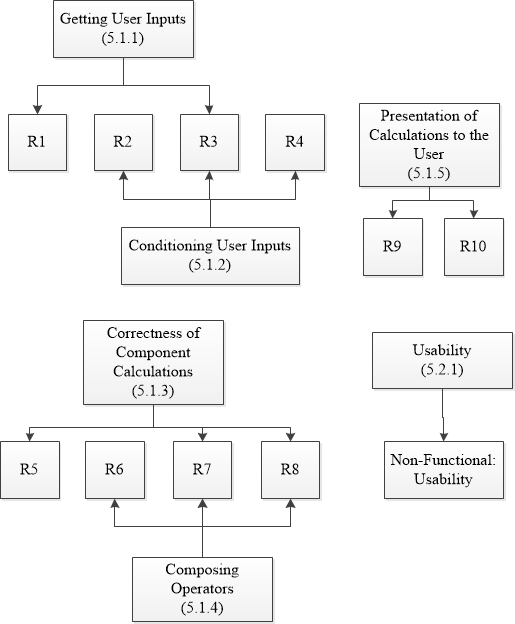
\includegraphics[width=0.66\textwidth]{figures/ReqToTest.png}
		}
		\caption{\label{Fig:req2tests} Traceability Graph Showing the 
		Connections Requirements and Test Suites}
	\end{center}
\end{figure}
				
\section{Unit Testing Plan}
		
As shown by the system test description (Section \ref{testplan_highlevel}), the 
system and integration testing of the \prognameAbbrv{} tool can be divided into 
several unique steps. This also has implications for specific function unit 
tests.

The general plan for unit testing is to use the same tests from the functional 
requirements (Section \ref{testplan_functional}) except that the expected 
inputs are provided by the human tester rather than the module that produces 
those values as outputs. For example if the $f(V)$ parsing function is 
expecting an error-checked $f(V)$ from the input module, the error-checked 
$f(V)$ would be provided by the human tester instead. If a manually synthesised 
input produces incorrect behaviours from a function, debugging strategies can 
be employed, including debugging statements and visual code inspections.

The unit testing stage is also the point where code coverage tools can be used 
to ensure that most lines of code are being tested by the integration and 
system tests. If code is not covered by the tests, it should be analysed to 
determine its usefulness and accessibility to the rest of the program.

Once a section of tests have been completed and there do not appear to be any 
immediate problems, the modules can be used in the functional requirement tests.

%\bibliographystyle{plainnat}

%\bibliography{SRS}

\newpage

\section{Appendix: Usability Survey Questions}
These surveys are designed to accompany the usability non-functional 
requirements tests (\ref{tests_nonfunctional_usability}).

\subsection{User Questions for Entering Values into the \prognameAbbrv{} 
Tool}
\label{questions_inputs}

\begin{enumerate}
	\item (Likert Scale) I was able to enter in the equation $f(V)$ in a format 
	that I was familiar with.
	\item (Likert Scale) I was able to enter in the equation $f(V)$ in a format 
	that I was expecting.
	\item (Likert Scale) I found it easy to enter the $f(V)$ equations into the 
	tool.
	\item (Likert Scale) I was able to enter in the domains $D(v)$ in a format 
	that I was familiar with.
	\item (Likert Scale) I was able to enter in the domains $D(v)$ in a format 
	that I was expecting.
	\item (Likert Scale) I found it easy to enter the domains $D(v)$ into the 
	tool.
	\item (Open Response) Do you have any suggestions for improving the 
	mathematical notation of the \prognameAbbrv{} tool?
\end{enumerate}

\subsection{User Questions for Using the \prognameAbbrv{} Tool GUI}
\label{questions_GUI}

\begin{enumerate}
	\item (Likert Scale) I found it easy to find the input mechanism for 
	entering $f(V)$ into the GUI.
	\item (Likert Scale) I found it easy to enter the $f(V)$ equations into the 
	GUI.
	\item (Likert Scale) I found it easy to find the input mechanism for 
	entering $D(v)$ into the GUI.
	\item (Likert Scale) I found it easy to enter the domains $D(v)$ into the 
	GUI.
	\item (Likert Scale) I found it easy to find the program's result for 
	$R(f(V))$ in the GUI.
	\item (Likert Scale) I found it easy to understand the program's result for 
	$R(f(V))$ in the GUI.
	\item (Likert Scale) I found it easy to understand the sequence of steps 
	required to use the \prognameAbbrv{} tool.
	\item (Open Response) Do you have any suggestions for improving the 
	process flow of the \prognameAbbrv{} tool?
\end{enumerate}


\end{document}